\documentclass[11pt]{article}

\usepackage[a4paper,
            bindingoffset=0.5cm,
            left=3cm,
            right=3cm,
            top=3cm,
            bottom=4cm,
            footskip=1.5cm]{geometry}
            
%
\usepackage[T1]{fontenc}
\usepackage{graphicx}
\usepackage{enumitem}
\usepackage{blindtext}
\usepackage{float}
%

\setcounter{secnumdepth}{3}

%%%%%%%%%%%%%%%%%%%%%
\title{\textbf{Critical Systems Lab - MESCC\\ Water Pumping Automated System}}
\date{ISEP, January 2024}
\author{Ricardo Mendes\\ 1201779
\and Arthur Gerbelli\\ 1220201}
%%%%%%%%%%%%%%%%%%%%%

\begin{document}

\maketitle              
\newpage
\tableofcontents
\newpage

%
\section{Introduction}

The current document, is the result of the work done during the first delivery of the CSLAB class.

The document is divided into three parts, each one of them focused on the evaluation topics: \textbf{requirements specification} documentation, \textbf{rationale for selected technology} and \textbf{list of physical sensor and/or actuator} used for the demo.

The system that we are modeling is a Water Pumping System (WPS) for two rainwater wells. These types of systems are essentially used to move water from a lower elevation to a higher one.

A Remote Status Station is also described in the document. Its main function is to give a level of observability of the WPS and to alert the \textit{maintenance team} for a possible failure.

There is also an additional feature. The status of the system should also be visible through a web server.


%%%
\section{Requirement Specification}

%%%
\subsection{Problem Domain}

%%%
\subsubsection{Stakeholder Needs}

Based on the system's description and some clarifications during the classes, we identified the following Stakeholder needs:

\begin{enumerate}[leftmargin=4em, font=\small, label=\textbf{SN-\arabic*}]
	\setlength\itemsep{.5em}
	\item 
		\begin{enumerate}[leftmargin=1.5em, font=\small, label=\textbf{.\arabic*:}]
		\setlength\itemsep{0em}	
		\item The water in the WPS must be pumped from a lower level to a higher one.
		\item Every WPS is an independent system; they don't have influence on each other.
		\end{enumerate}
	\item 
		\begin{enumerate}[leftmargin=1.5em, font=\small, label=\textbf{.\arabic*:}]
		\setlength\itemsep{0em}	
		\item The status of each element of the wet well needs to be displayed in a Remote Status Station (RSS). 
		\item The RSS must display the water level, the pump status, an alarme and a button to disable the alarm.
		\item The alarm must be ON when a problem in the system is identified.
		\end{enumerate}
		
	\item The status information must be accessible through a web page.
\end{enumerate}

\noindent
\textbf{SN-1} is WPS specific, \textbf{SN-2} is RSS specific and \textbf{SN-3} is Web Server specific.

%%%
\subsubsection{System Context}

For a better understanding of the system, we developed an external view, and so, identified external entities that do not belong to the system but interact with it. The following diagram is the output of this analysis:

\begin{figure}[H]
  \centering
  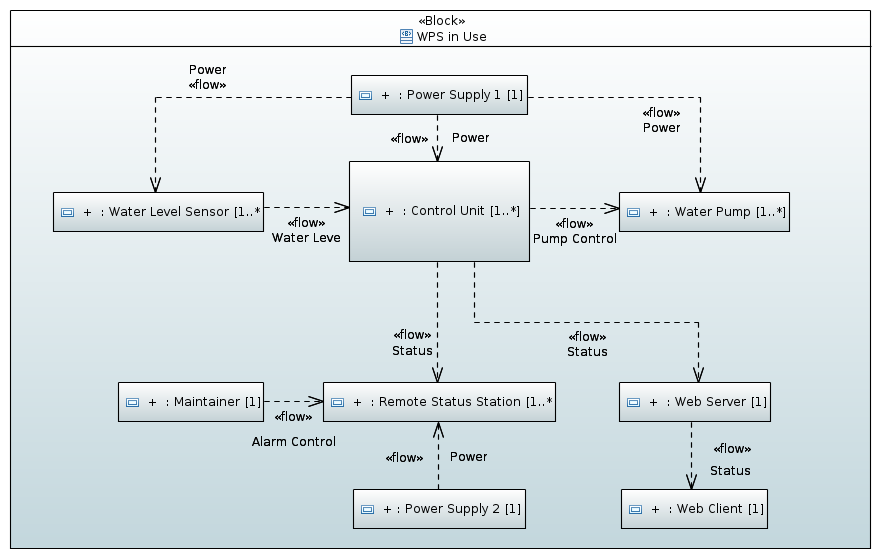
\includegraphics[width=300px]{../diagrams/system-context-01.png}
  \caption{System Context}
  \label{fig:System Context}
\end{figure}

Although some elements represented in the diagram are part of the WPS (sensor, control unit, pump and RSS), we divide them into subsystems with their own responsibilities and interactions. 

By decoupling the WPS responsibilities, we are simplifying it and turning the critical system requirements easier to grasp and model. 

The main identified external entities are: \textbf{Power Supply}, \textbf{Maintenance Team} and \textbf{Web Client}. 

Please notice the independent Power Supply for the Control Unit and the RSS as a way to deal with the critical requirements.

%%%
\subsubsection{Use Cases}

By analyzing the Stakeholder Needs, we can see that the main goal of the WPS is to control the water level inside the wet well. This goal can be captured in the model as the \textit{"Control Water Level"} use case of the \textit{Control Unit In Use} system context. 

\begin{figure}[H]
  \centering
  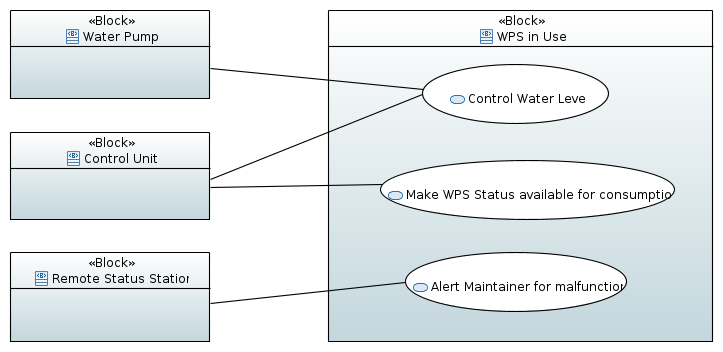
\includegraphics[width=300px]{../diagrams/use-cases-01.png}
  \caption{Use Case diagram}
  \label{fig:Use Case1}
\end{figure}

A closer look at the use case \textit{"Control Water Level"} gave rise to the below activity diagram. No alternative scenario was modeled.

\begin{figure}[H]
  \centering
  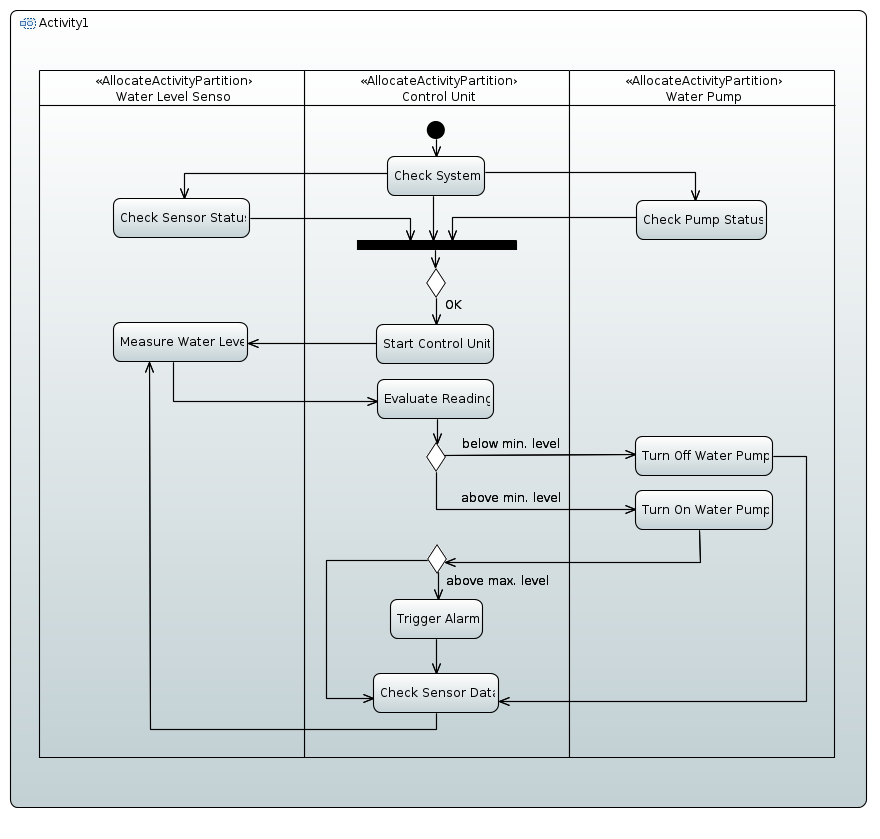
\includegraphics[width=300px]{../diagrams/use-case-activity-diagram-01.png}
  \caption{Use Case Activity diagram}
  \label{fig:Use Case2}
\end{figure}

%%%
\subsubsection{Measure of Effectiveness}

To be able to describe the performance of the system, some quantifiable characteristics of the WPS were identified:

\begin{itemize}
\setlength\itemsep{0em}
  \item Energy Consumption in \textit{kilowatts per hour}
  \item Wet Well Capacity in \textit{cubic meters};
  \item Water Inflow in \textit{liters per second};
  \item Water Outflow in \textit{liters per second}.
\end{itemize}

\begin{figure}[H]
  \centering
  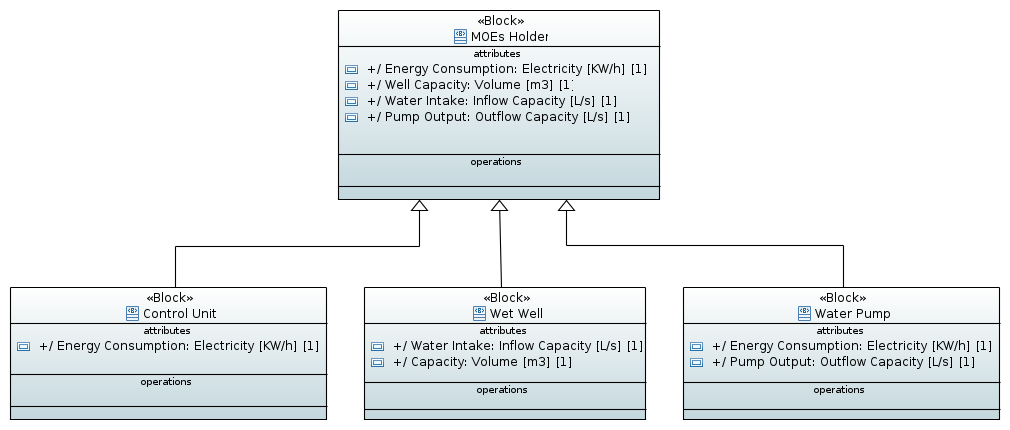
\includegraphics[width=300px]{../diagrams/measure-of-effectiveness.png}
  \caption{Measure of Effectiveness diagram}
  \label{fig:MoE}
\end{figure}

As illustrated, each characteristic can be related to a specific element of the WPS.

%%%
\subsubsection{Functional Analysis}

For the functional analysis, we only focused our attention to the Control Unit; the most critical of the subsystems.

\begin{figure}[H]
  \centering
  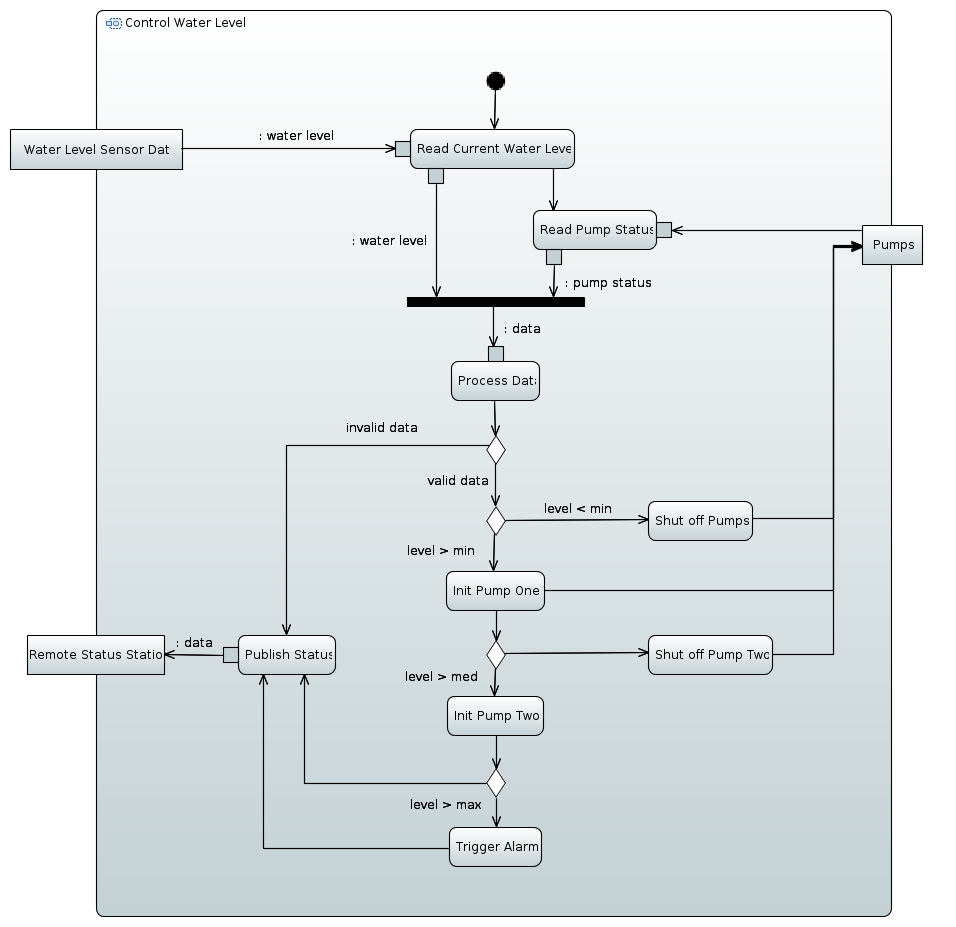
\includegraphics[width=300px]{../diagrams/functional-analysis-wps.png}
  \caption{Functional Analysis diagram}
  \label{fig:Functional Analysis}
\end{figure}

For a reliable \textit{Water Level Control}, the Control Unit needs to be able to read data from the sensors and also get the current status of the water pumps.

This data is used to decide the correct behavior - turn on or off the water pumps - and publish the system's status to be consumed by the RSS.

The system's status also has the information that can trigger an alarm on the RSS side.

%%%
\subsubsection{Conceptual Subsystems}

After identifying conceptual subsystems during the functional analysis, we tried to capture the communication between them. This was achieved by pinpointing  the inputs and outputs of those subsystems.

\begin{figure}[H]
\centering
\begin{minipage}{.5\linewidth}
  \centering
  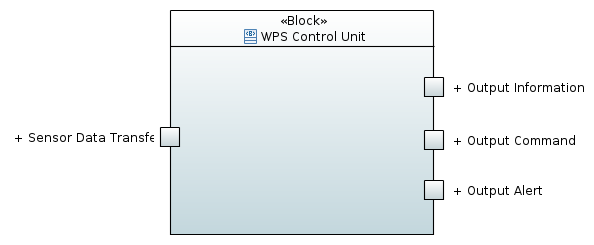
\includegraphics[width=150px]{../diagrams/conceptual-subsystem-communication-wps.png}
  \caption{Communication WPS}
  \label{fig:Conceptual Subsystem 1}
\end{minipage}%
\begin{minipage}{.5\linewidth}
  \centering
  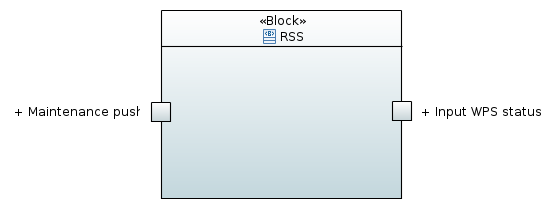
\includegraphics[width=150px]{../diagrams/conceptual-subsystem-communication-rss.png}
  \caption{Communication RSS}
  \label{fig:Conceptual Subsystem 2}
\end{minipage}
\end{figure}

In the diagrams above, we analyzed the WSP Control Unit and the RSS.

%%%
\subsection{Solution Domain}

%%%
\subsubsection{System Requirements}

These system's requirements were expressed using the EARS method. The objective of this approach is to state in a concise, feasible and traceable way what the system must do and its limitations.

All the requirements below are functional requirements. non-functional requirements are not being taken into account. These are specified on a later chapter.

\begin{enumerate}[leftmargin=4em, font=\small, label=\textbf{SR-\arabic*}]
	\setlength\itemsep{.5em}
	\item 
		\begin{enumerate}[leftmargin=1.5em, font=\small, label=\textbf{.\arabic*:}]
		\setlength\itemsep{0em}
		\item While the water level is above the minimum level, WPS shall have a pump working.
		\item When the water level is below minimum level, WPS shall have all pumps stopped.
		\item If the water level is above the maximum level, then the WPS shall trigger an alarm at the Remote Status Station (RSS).
		\item A second pump shall be turned on only when the water level is above 2/3 the maximum water level.
		\item When only one pump is available, the maximum water level shall be reduced to 2/3.
		\end{enumerate}
	\item
		\begin{enumerate}[leftmargin=1.5em, font=\small, label=\textbf{.\arabic*:}]
		\setlength\itemsep{0em}
		\item The status of all WPS shall be displayed on all RSS.
		\item If the alarm is ON, the button in the RSS shall only disable it.
		\end{enumerate}
	\item The status of all WPS shall be visible on a web page.

\end{enumerate}

\noindent
\textbf{SR-1} is WPS specific, \textbf{SR-2} is RSS specific and \textbf{SR-3} is Web Server specific.

The requirements are the output of the previous analysis. If we look at the functional analysis made for the \textit{"Control Water Level"} use case, we can clearly map it to the \textbf{SR-1}. 

\newpage

%%%
\subsubsection{Traceability to Stakeholder Needs}

In order to confirm that the output of the problem domain model is being followed, we need to establish traceability relationships. 

In this particular case, we jumped the system's functions during the white-box analysis, and focused on the identified requirements and confirmed that they respond to the Stakeholders needs.

\begin{figure}[H]
  \centering
  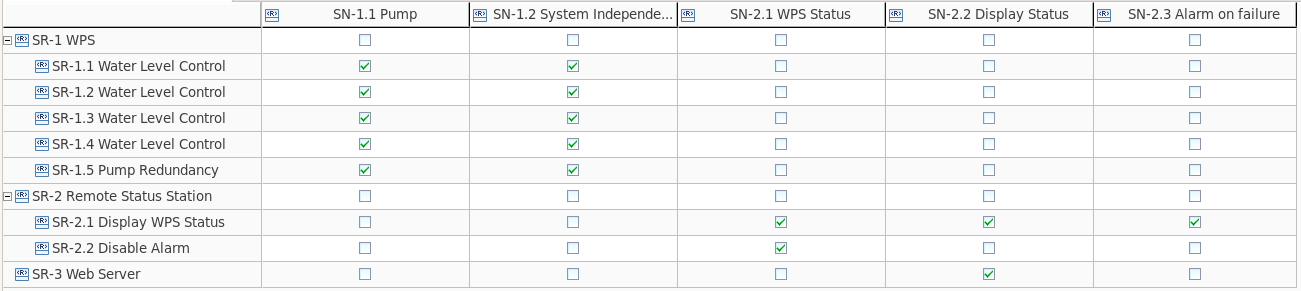
\includegraphics[width=\linewidth]{../diagrams/traceability.png}
  \caption{Traceability to Stakeholder Needs}
  \label{fig:Traceability}
\end{figure}

As illustrated, the requirements are answering the Stakeholder needs.

%%%
\subsubsection{System Structure}

Having the system requirements, we can start thinking about the logical architecture of the WPS.

In this case, the subsystem of the solution domain, don't differ from the subsystems identified in the problem domain. 

Although the Web Server was not explicitly described during the problem domain, this fact only happened because of a more focused analysis of the critical parts.

\begin{figure}[H]
  \centering
  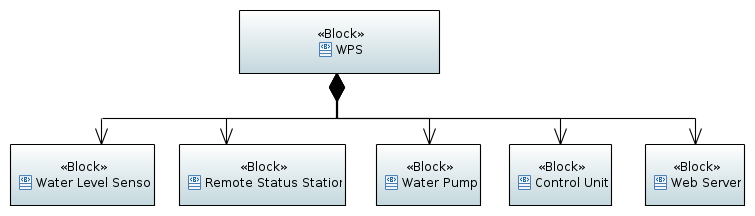
\includegraphics[width=300px]{../diagrams/system-structure.png}
  \caption{System Structure Diagram}
  \label{fig:System Structure Diagram}
\end{figure}

\newpage

%%%
\subsubsection{System Behavior}
\textit{Mealy Finite State Machine} to describe the behavior of the WPS.

The only input to the machine is the current water level. The state of the machine changes according to these values.

There are two main states are ON and OFF, corresponding to water being or not pumped outside the well. If the water level in above the minimum, a water pump must be working (ON LOW). Depending on the levels above minimum, we can have a second pump working with (ON HIGH) or without (ON ALERT) an alert being triggered.

The state machine, beneath, models this behavior.

\begin{figure}[H]
  \centering
  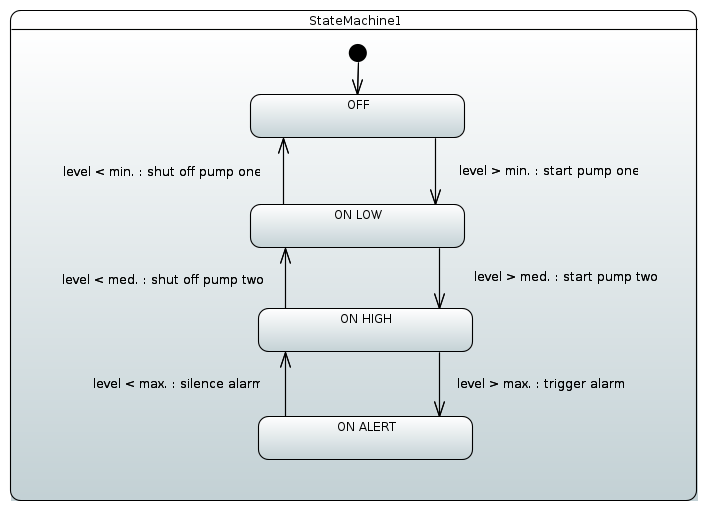
\includegraphics[width=300px]{../diagrams/state-machine-wps.png}
  \caption{State Machine}
  \label{fig:State Machine}
\end{figure}


%%%
%%%
%%%
\subsection{Analysis of safety and reliability}

Given that we are dealing with a critical system, the analysis of safety and reliability as bigger impact on the implementation of the solution.

\begin{enumerate}[leftmargin=4em, font=\small, label=\textbf{H-\arabic*:}]
	\setlength\itemsep{.5em}
	\item 
		\begin{itemize}
		\setlength\itemsep{0em}
        		\item \textbf{Description:} One of the pumps stops working.
		\item Cause: Mechanical problem.
    		\item Effect: Lost of redundancy and reduction of system performance.
    		\item \textbf{Mitigation:} Reduce the maximum water level to 2/3 and trigger alarm.
		\end{itemize}
	\item 
		\begin{itemize}
		\setlength\itemsep{0em}
    		\item \textbf{Description:} The two level sensors give contradictory readings, i.e. one above max and one below min.
		\item Cause: Sensor malfunction, connection issues.
    		\item Effect: Inappropriate system behavior. 
    		\item \textbf{Mitigation:} Choose a worst case or compare with the last reading to find the fault. Always trigger the alarm.
		\end{itemize}
	\item 
		\begin{itemize}
		\setlength\itemsep{0em}
    		\item \textbf{Description:} Power shortage.
		\item Cause: Multiple causes
    		\item Effect: Complete failure of the system.
    		\item \textbf{Mitigation:} RSS with independente power supply and trigger alarm.
		\end{itemize} 
	\item 
		\begin{itemize}
		\setlength\itemsep{0em}
    		\item \textbf{Description:} Both pumps stopped working.
		\item Cause: Mechanical problem.
    		\item Effect: Complete failure of the system.
    		\item \textbf{Mitigation:} Trigger alarm.
		\end{itemize} 
	\item 
		\begin{itemize}
		\setlength\itemsep{0em}
    		\item \textbf{Description:} RSS are not getting information from WPS.
		\item Cause: Connection issues or Messagem broker stoped working.
    		\item Effect: Unknown status of the system.
    		\item \textbf{Mitigation:} Implement a cluter of MQTT Brokers or remove this single point of failure by adopting DDS.
		\end{itemize} 
	\item 
		\begin{itemize}
		\setlength\itemsep{0em}
    		\item \textbf{Description:} RSS stops working.
		\item Cause: Malfunction.
    		\item Effect: Unknown WPS status.
    		\item \textbf{Mitigation:} Have redundancy by having multiple RSS and each one displaying all statuses from all WPS.
		\end{itemize} 
	\item 
		\begin{itemize}
		\setlength\itemsep{0em}
    		\item \textbf{Description:} A pump doesn't turn OFF when the water level in bellow minimum.
			\item Cause: Mechanical problem.
    		\item Effect: Pump overheating and complete failure.
    		\item \textbf{Mitigation:} Trigger alarm.
		\end{itemize} 
\end{enumerate}

Most of the hazards here listed could be handled as non-functional requirements. Because of that, a more detailed description of some of them is needed.
\\[12pt]
\textbf{H-1} and \textbf{H-4} touches on the redundancy of the water pumps. Because having an unused water pump would mean a reduced performance of the system, we choose to use the two pumps even when the system is healthy. The second pump is only used when the water level is high. If, for some reason, one of the pumps is not working, the system will reduce the max capacity of the well and trigger an alarm to alert the maintenance team.
\\[12pt]
\textbf{H-2} is interesting because introduces a problem that cannot be answered with a reliable voting system. If the reading of both sensor are too unequal, there must be a way to distinguish between the wrong and the correct data. There are three possible ways to deal with the issues: choose a master and a slave sensor, retain the previous input and compare it with the current one, or choose the worst case.
\\[12pt]
\textbf{H-3} and \textbf{H-6} illustrates the importance of the RSS. During a localized power shortage on the well, the RSS should not be affected and so, still be able to alert the maintenance team. Having two RSS in the building also assures redundancy, specially if they have separated power supplies.
\\[12pt]
\textbf{H-5} is sensible to a special limitation of having only one system dealing with the main communication. A single MQTT broker is also a single point of failure that could jeopardize the whole system. Having a cluster of brokers or using a middleware like DDS is a way to mitigate or even remove completely this risk.

\newpage
%%%
\section{Selected Technologies}

Before describing the selected technologies, we want to emphasize that the selection was made on the basis of this being an academic exercise and that at the end a demo must be presented using microcontrollers, simple sensors and actuators.

Here are the selected communication technologies:

\begin{itemize}
	\item \textbf{MQTT} is a lightweigh messaging protocol specially developed for the IoT. It is based on the publish/subscribe paradigm and is a perfect choise for a small code footprint and reduced network bandwidth.
	
The MQTT protocol was not design to deal with authentication or authorization standards in a possible effort to avoid weaken some of its strengths i.e. low bandwidth usage, speed and low power consumption.

Not being encrypted, MQTT supports itself on TLS/SSL for security encryption as we already wrote in a previous chapter. MQTT is not trust symmetrical and by using SSL certificates the client can have some assurance that the 
server is legit.

In conclusion, the protocol includes recommendations for its implementation in application so to ensure a level of security according to today’s standards

Although the above-mentioned security issues, the main communication protocol between sensors and control units will be MQTT. Because the status of the system will be displayed in the RSS and also on a web page. The publish/subscribe method is ideal when multiple consumer are in play.

	\item \textbf{TCP} will be used as a fallback in case no data is being made available by the MQTT broker. If a sensor fails and the control unit confirms that no message is being sent, it can always make a request to the sensor the query about its status.

TCP is also the main communication protocol of the IP suite. Some of the communication in the network that we will use for the demo will use it on a higher level, i.e. HTTP.

	\item \textbf{HTTP and REST}. The required web page, that displays the status of the system, almost forces us to use the HTTP protocol during the client-server communication. On the server side, an API following the REST guidelines will be implemented.

	\item \textbf{JSON}. The data between Web client and Web server will be made available in JSON. This text format is ideal for the demo because of being widely uses, language independent and easily parsed by all the main programming languages.

	Binary formats like Parquet or Protobuf could have being an interesting alternative, but the overhead of the implementation is not realistic for this exercise.
	
\end{itemize}

Here are the selected programming languages:

\begin{itemize}
	\item \textbf{C}. All the main services will be written in C. This enables us a smaller code footprint an a greater control of the hardware resources.
	\item \textbf{Assembly} is a requirement of the exercise and will be used to simulate the Water Level Sensors.
	\item \textbf{Python} is certainly not used in critical systems. Because of that, this programming language will be used to implement the HTTP server that doesn't have any critical requirement.
	\item HTML is not a programming language! But for the sake of completeness, this markup language will be used to use a common browser as our Web client.
\end{itemize}

To have a better overview of the proposed implementation of the system, we elaborated a deployment diagram with all the discussed services:

\begin{figure}[H]
  \centering
  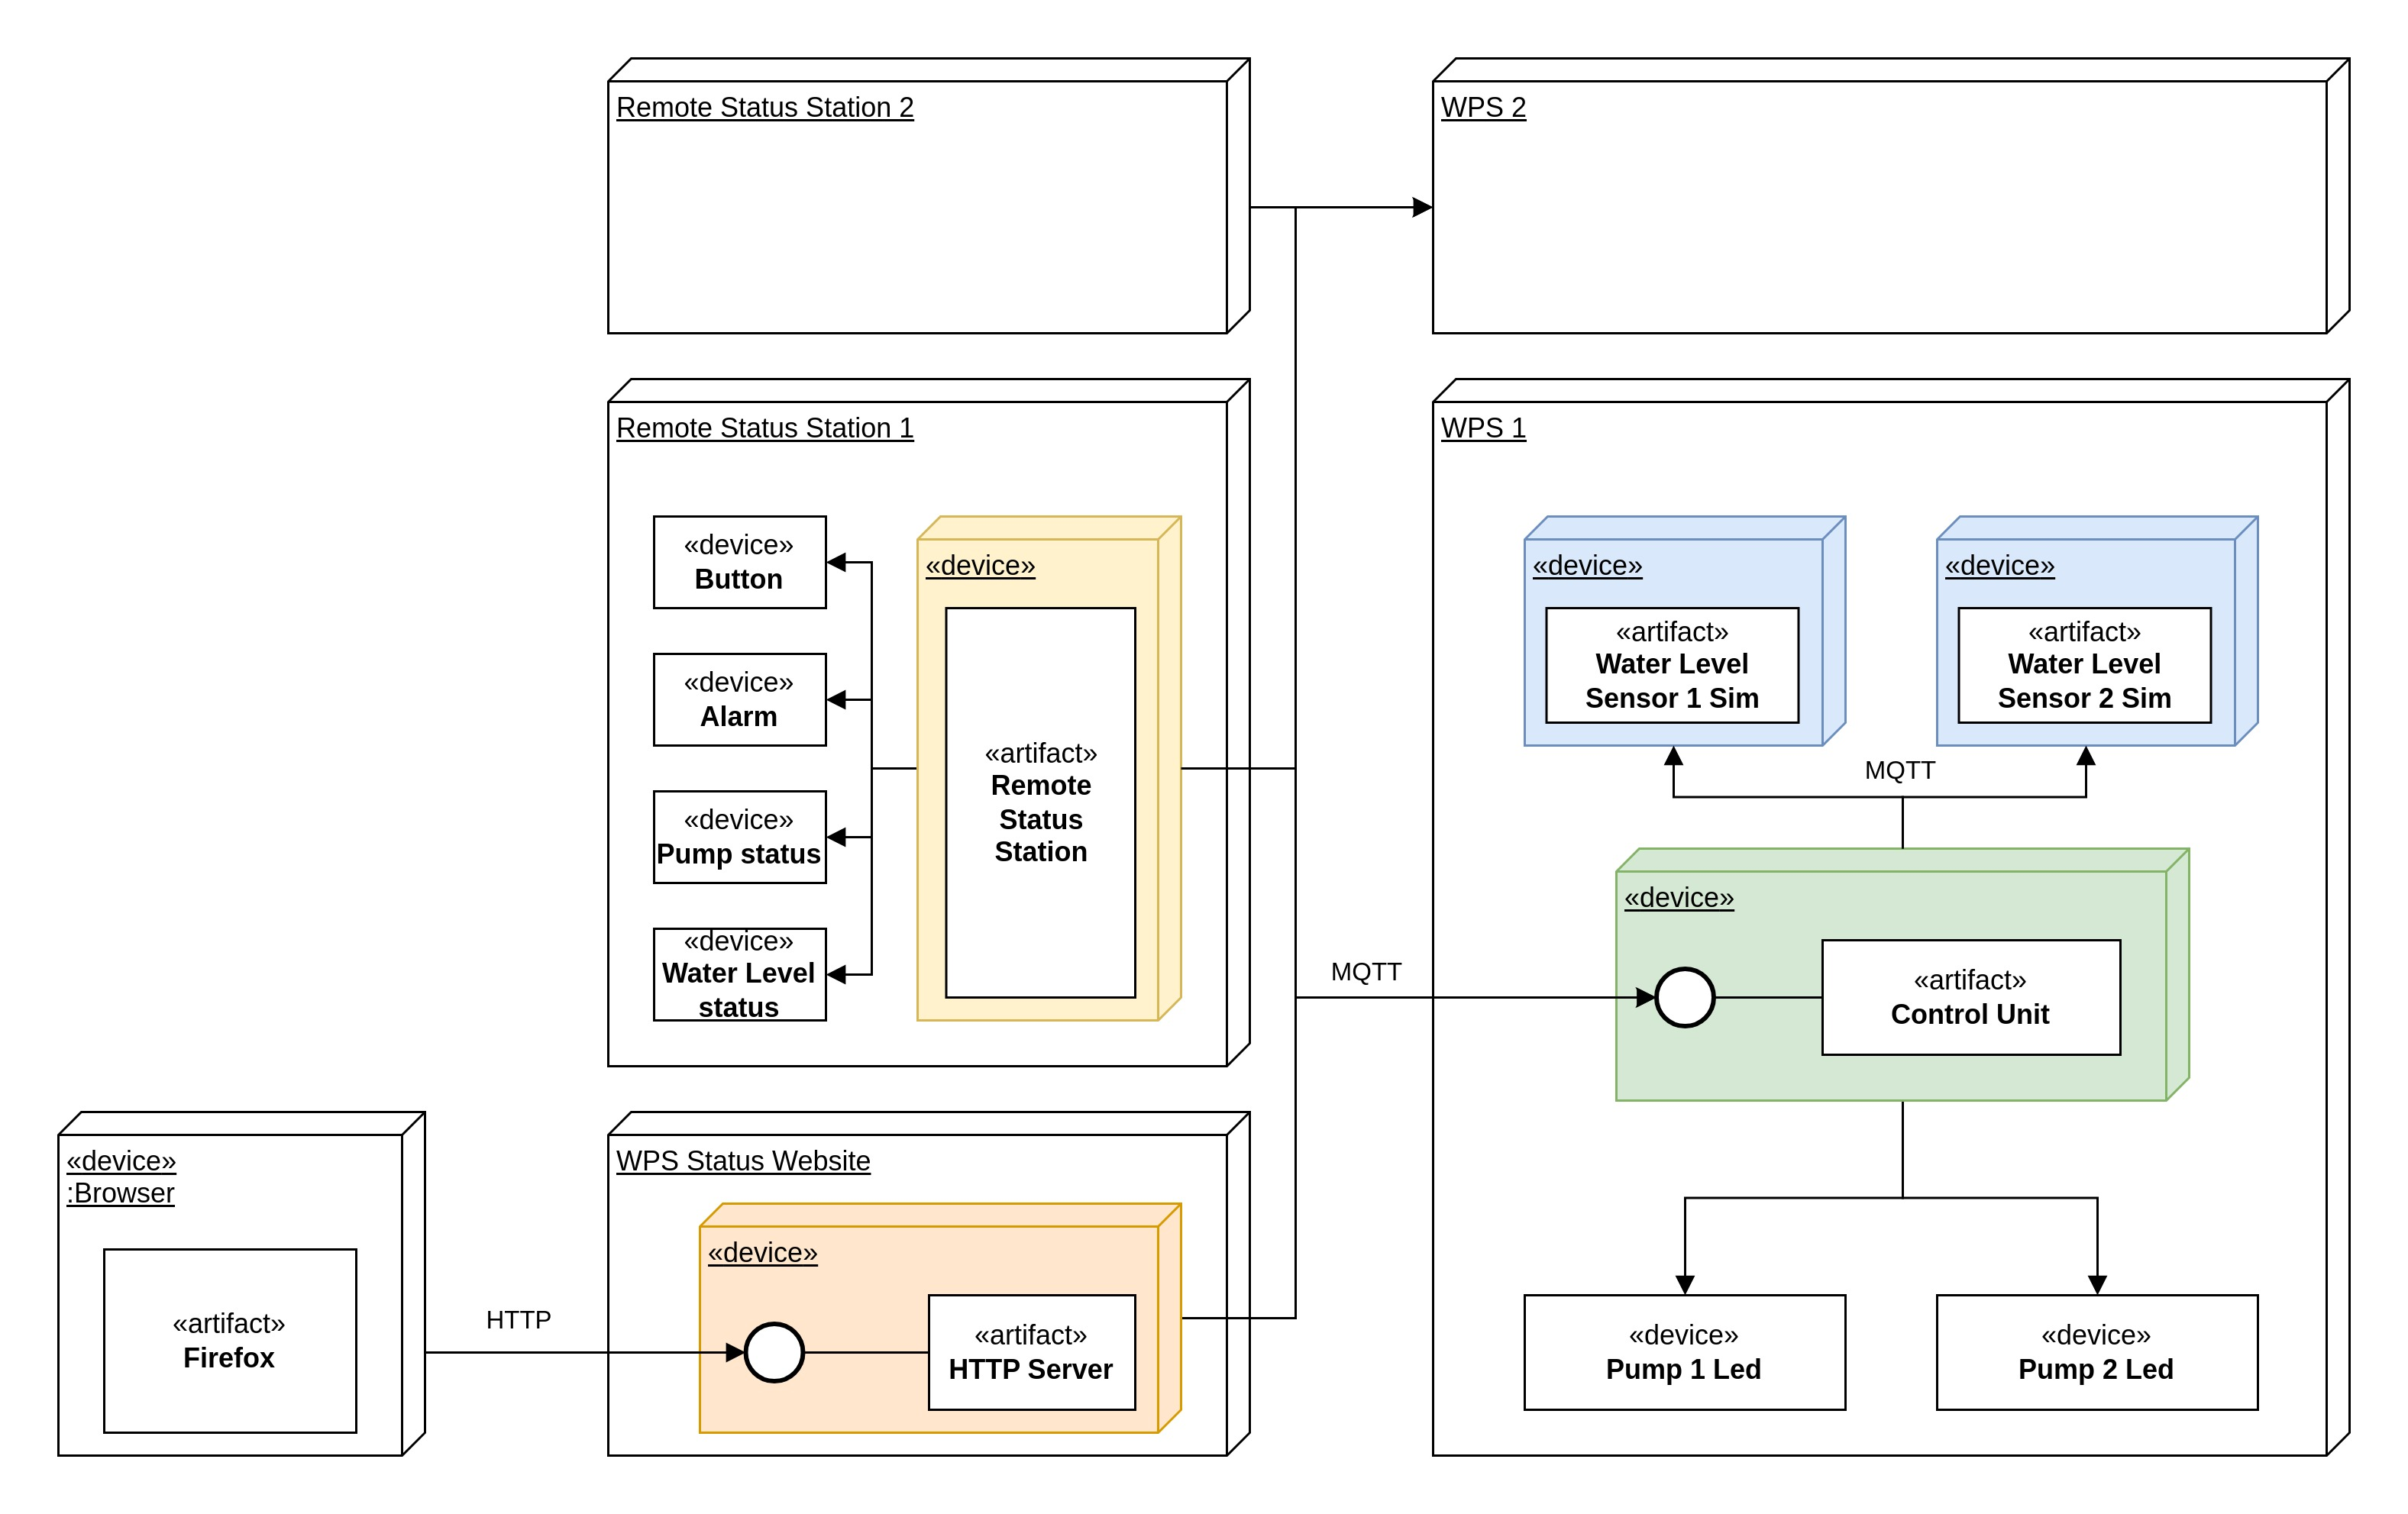
\includegraphics[width=\linewidth]{../diagrams/deployment-diagram-WPS.jpg}
  \caption{Deployment diagram}
  \label{fig:Deployment Diagram}
\end{figure}

\newpage
%%%
\section{List of physical sensors/actuators}

\begin{figure}[H]
  \centering
  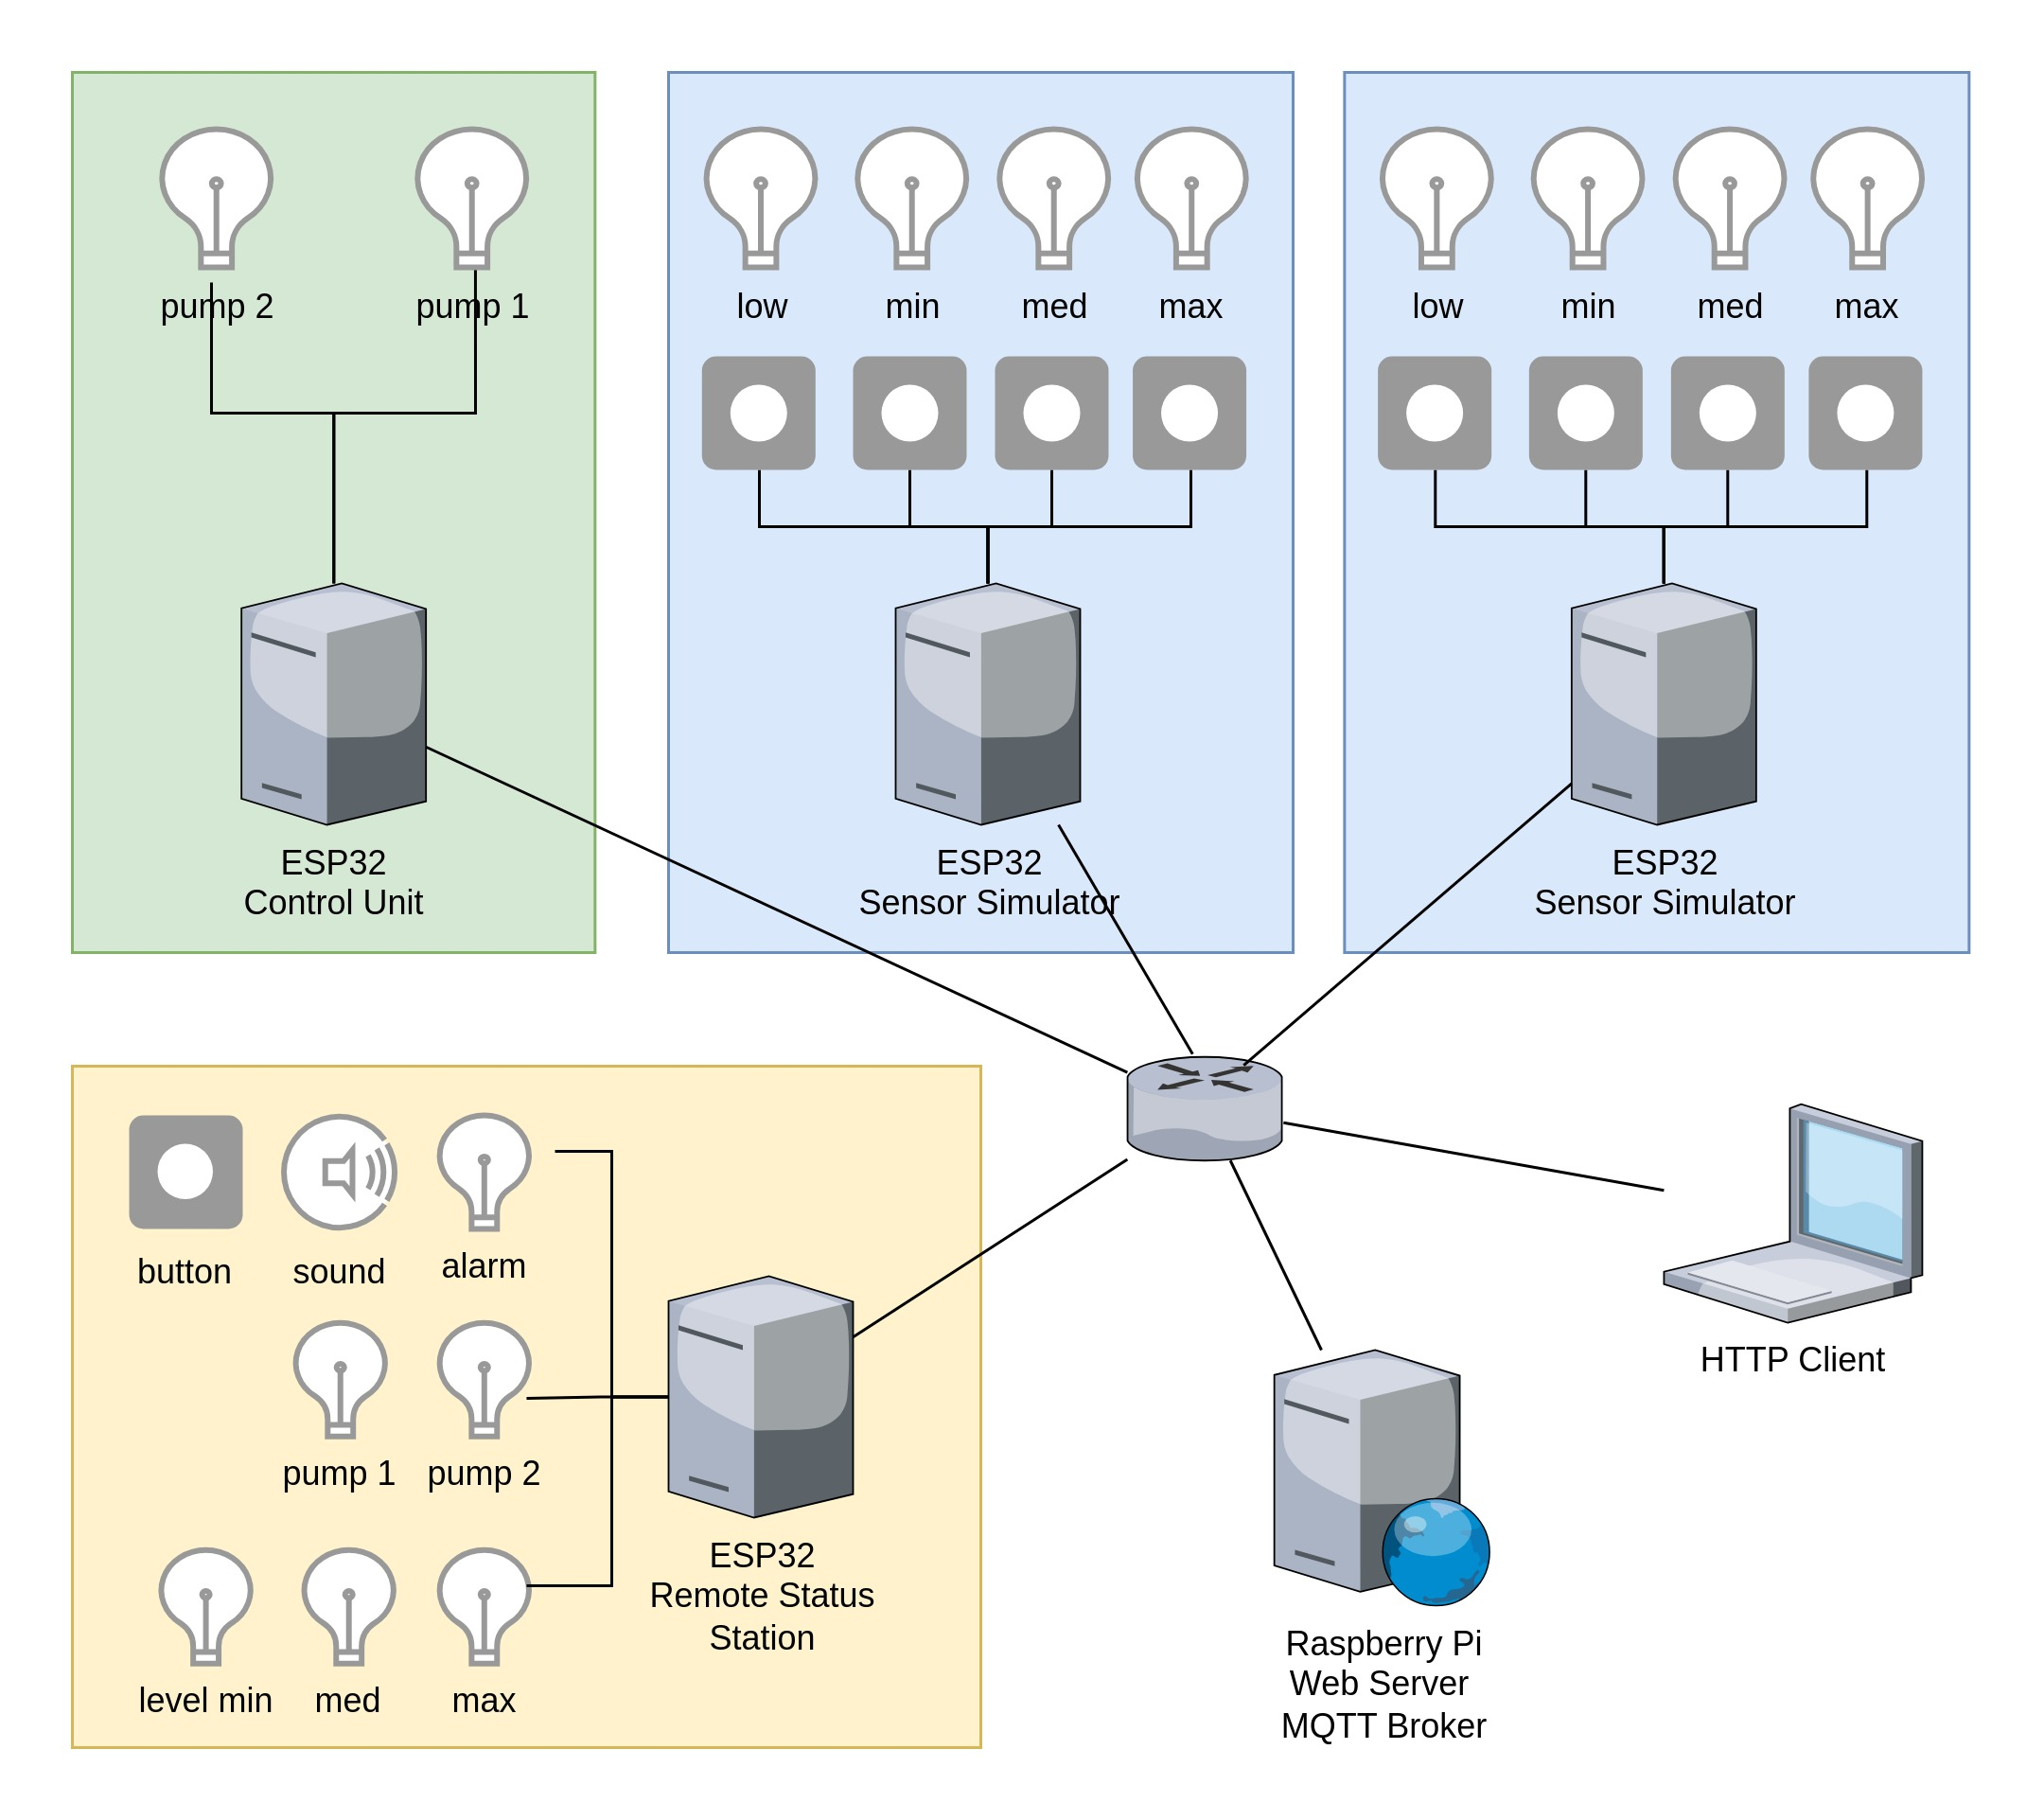
\includegraphics[width=300px]{../diagrams/network-diagram-WPS.jpg}
  \caption{Network diagram}
  \label{fig:Network1 Diagram}
\end{figure}

\end{document}
